% Options for packages loaded elsewhere
\PassOptionsToPackage{unicode}{hyperref}
\PassOptionsToPackage{hyphens}{url}
%
\documentclass[
]{article}
\usepackage{amsmath,amssymb}
\usepackage{lmodern}
\usepackage{iftex}
\ifPDFTeX
  \usepackage[T1]{fontenc}
  \usepackage[utf8]{inputenc}
  \usepackage{textcomp} % provide euro and other symbols
\else % if luatex or xetex
  \usepackage{unicode-math}
  \defaultfontfeatures{Scale=MatchLowercase}
  \defaultfontfeatures[\rmfamily]{Ligatures=TeX,Scale=1}
\fi
% Use upquote if available, for straight quotes in verbatim environments
\IfFileExists{upquote.sty}{\usepackage{upquote}}{}
\IfFileExists{microtype.sty}{% use microtype if available
  \usepackage[]{microtype}
  \UseMicrotypeSet[protrusion]{basicmath} % disable protrusion for tt fonts
}{}
\makeatletter
\@ifundefined{KOMAClassName}{% if non-KOMA class
  \IfFileExists{parskip.sty}{%
    \usepackage{parskip}
  }{% else
    \setlength{\parindent}{0pt}
    \setlength{\parskip}{6pt plus 2pt minus 1pt}}
}{% if KOMA class
  \KOMAoptions{parskip=half}}
\makeatother
\usepackage{xcolor}
\usepackage[margin=1in]{geometry}
\usepackage{color}
\usepackage{fancyvrb}
\newcommand{\VerbBar}{|}
\newcommand{\VERB}{\Verb[commandchars=\\\{\}]}
\DefineVerbatimEnvironment{Highlighting}{Verbatim}{commandchars=\\\{\}}
% Add ',fontsize=\small' for more characters per line
\usepackage{framed}
\definecolor{shadecolor}{RGB}{248,248,248}
\newenvironment{Shaded}{\begin{snugshade}}{\end{snugshade}}
\newcommand{\AlertTok}[1]{\textcolor[rgb]{0.94,0.16,0.16}{#1}}
\newcommand{\AnnotationTok}[1]{\textcolor[rgb]{0.56,0.35,0.01}{\textbf{\textit{#1}}}}
\newcommand{\AttributeTok}[1]{\textcolor[rgb]{0.77,0.63,0.00}{#1}}
\newcommand{\BaseNTok}[1]{\textcolor[rgb]{0.00,0.00,0.81}{#1}}
\newcommand{\BuiltInTok}[1]{#1}
\newcommand{\CharTok}[1]{\textcolor[rgb]{0.31,0.60,0.02}{#1}}
\newcommand{\CommentTok}[1]{\textcolor[rgb]{0.56,0.35,0.01}{\textit{#1}}}
\newcommand{\CommentVarTok}[1]{\textcolor[rgb]{0.56,0.35,0.01}{\textbf{\textit{#1}}}}
\newcommand{\ConstantTok}[1]{\textcolor[rgb]{0.00,0.00,0.00}{#1}}
\newcommand{\ControlFlowTok}[1]{\textcolor[rgb]{0.13,0.29,0.53}{\textbf{#1}}}
\newcommand{\DataTypeTok}[1]{\textcolor[rgb]{0.13,0.29,0.53}{#1}}
\newcommand{\DecValTok}[1]{\textcolor[rgb]{0.00,0.00,0.81}{#1}}
\newcommand{\DocumentationTok}[1]{\textcolor[rgb]{0.56,0.35,0.01}{\textbf{\textit{#1}}}}
\newcommand{\ErrorTok}[1]{\textcolor[rgb]{0.64,0.00,0.00}{\textbf{#1}}}
\newcommand{\ExtensionTok}[1]{#1}
\newcommand{\FloatTok}[1]{\textcolor[rgb]{0.00,0.00,0.81}{#1}}
\newcommand{\FunctionTok}[1]{\textcolor[rgb]{0.00,0.00,0.00}{#1}}
\newcommand{\ImportTok}[1]{#1}
\newcommand{\InformationTok}[1]{\textcolor[rgb]{0.56,0.35,0.01}{\textbf{\textit{#1}}}}
\newcommand{\KeywordTok}[1]{\textcolor[rgb]{0.13,0.29,0.53}{\textbf{#1}}}
\newcommand{\NormalTok}[1]{#1}
\newcommand{\OperatorTok}[1]{\textcolor[rgb]{0.81,0.36,0.00}{\textbf{#1}}}
\newcommand{\OtherTok}[1]{\textcolor[rgb]{0.56,0.35,0.01}{#1}}
\newcommand{\PreprocessorTok}[1]{\textcolor[rgb]{0.56,0.35,0.01}{\textit{#1}}}
\newcommand{\RegionMarkerTok}[1]{#1}
\newcommand{\SpecialCharTok}[1]{\textcolor[rgb]{0.00,0.00,0.00}{#1}}
\newcommand{\SpecialStringTok}[1]{\textcolor[rgb]{0.31,0.60,0.02}{#1}}
\newcommand{\StringTok}[1]{\textcolor[rgb]{0.31,0.60,0.02}{#1}}
\newcommand{\VariableTok}[1]{\textcolor[rgb]{0.00,0.00,0.00}{#1}}
\newcommand{\VerbatimStringTok}[1]{\textcolor[rgb]{0.31,0.60,0.02}{#1}}
\newcommand{\WarningTok}[1]{\textcolor[rgb]{0.56,0.35,0.01}{\textbf{\textit{#1}}}}
\usepackage{graphicx}
\makeatletter
\def\maxwidth{\ifdim\Gin@nat@width>\linewidth\linewidth\else\Gin@nat@width\fi}
\def\maxheight{\ifdim\Gin@nat@height>\textheight\textheight\else\Gin@nat@height\fi}
\makeatother
% Scale images if necessary, so that they will not overflow the page
% margins by default, and it is still possible to overwrite the defaults
% using explicit options in \includegraphics[width, height, ...]{}
\setkeys{Gin}{width=\maxwidth,height=\maxheight,keepaspectratio}
% Set default figure placement to htbp
\makeatletter
\def\fps@figure{htbp}
\makeatother
\setlength{\emergencystretch}{3em} % prevent overfull lines
\providecommand{\tightlist}{%
  \setlength{\itemsep}{0pt}\setlength{\parskip}{0pt}}
\setcounter{secnumdepth}{-\maxdimen} % remove section numbering
\ifLuaTeX
  \usepackage{selnolig}  % disable illegal ligatures
\fi
\IfFileExists{bookmark.sty}{\usepackage{bookmark}}{\usepackage{hyperref}}
\IfFileExists{xurl.sty}{\usepackage{xurl}}{} % add URL line breaks if available
\urlstyle{same} % disable monospaced font for URLs
\hypersetup{
  pdftitle={project},
  hidelinks,
  pdfcreator={LaTeX via pandoc}}

\title{project}
\author{}
\date{\vspace{-2.5em}2023-01-09}

\begin{document}
\maketitle

\begin{Shaded}
\begin{Highlighting}[]
\FunctionTok{rm}\NormalTok{(}\AttributeTok{list =} \FunctionTok{ls}\NormalTok{())}
\FunctionTok{library}\NormalTok{(plyr)}
\FunctionTok{library}\NormalTok{(tidyr)}
\FunctionTok{detach}\NormalTok{(package}\SpecialCharTok{:}\NormalTok{plyr) }
\FunctionTok{library}\NormalTok{(dplyr)}
\FunctionTok{library}\NormalTok{(lubridate)}
\FunctionTok{library}\NormalTok{(forcats)}
\FunctionTok{library}\NormalTok{(stringr)}
\FunctionTok{library}\NormalTok{(readr)}
\FunctionTok{library}\NormalTok{(boot)}
\FunctionTok{library}\NormalTok{(caret)}
\FunctionTok{library}\NormalTok{(kernlab)}

\NormalTok{data\_all }\OtherTok{\textless{}{-}} \FunctionTok{read\_csv}\NormalTok{(}\StringTok{\textquotesingle{}Crimes\_2019.csv\textquotesingle{}}\NormalTok{,}\AttributeTok{show\_col\_types =} \ConstantTok{FALSE}\NormalTok{)}



\NormalTok{data }\OtherTok{\textless{}{-}}\NormalTok{ data\_all }\SpecialCharTok{\%\textgreater{}\%} \FunctionTok{select}\NormalTok{(}\SpecialCharTok{{-}}\FunctionTok{c}\NormalTok{(ID, }\StringTok{\textasciigrave{}}\AttributeTok{Case Number}\StringTok{\textasciigrave{}}\NormalTok{, Block, IUCR, Description, Beat, Ward, }\StringTok{\textasciigrave{}}\AttributeTok{Community Area}\StringTok{\textasciigrave{}}\NormalTok{, }\StringTok{\textasciigrave{}}\AttributeTok{Updated On}\StringTok{\textasciigrave{}}\NormalTok{, Latitude, Longitude, Location, Year, }\StringTok{\textasciigrave{}}\AttributeTok{Location Description}\StringTok{\textasciigrave{}}\NormalTok{))}

\NormalTok{data}\SpecialCharTok{$}\NormalTok{Date }\OtherTok{\textless{}{-}} \FunctionTok{parse\_datetime}\NormalTok{(data}\SpecialCharTok{$}\NormalTok{Date, }\AttributeTok{format =} \StringTok{"\%m/\%d/\%Y \%I:\%M:\%S \%p"}\NormalTok{)}
\end{Highlighting}
\end{Shaded}

\section{Binary Classification}

In this section we attempt to fit a binary classification model, to
predict given certain information whether the crime would lead to an
arrest or not. Choosing only to use 2019 data, due to scale of the data
set (leaving us with roughly 250,000 observations), as data recorded
after is affected strongly by COVID.

The features we choose to include in this model are:
\[\mathbf{x} = \texttt{(Domestic, Primary Type, Day, Time, Week Day, District})\]
We choose \texttt{Primary Type} over \texttt{FBI Code} to determine the
type of crime as during our EDA we found inconsistencies with the
classification of \texttt{FBI Code}. With \texttt{Primary Type}, we
merge uncommon levels of our factor variable into the level
\texttt{OTHER",\ in\ which\ we\ also\ include\ the\ pre-existing\ crime\ type}OTHER
OFFENSE''.

For temporal data we include \texttt{Week Day} as a factor variable,
encoding date using \texttt{Day} (1-365) and \texttt{Time} as a numeric
character between 0-1.

In order to include spatial information, we consider the
\texttt{District} variable. We observe that all districts experience
reasonable numbers of crimes to be incorporated into analysis, with the
exception of District 031.

While including more information might improve our models, during our
EDA we found the inclusion of highly correlated variables to improve the
model insignificantly while drastically increasing computational time.

\begin{Shaded}
\begin{Highlighting}[]
\NormalTok{othering }\OtherTok{\textless{}{-}} \ControlFlowTok{function}\NormalTok{(factor\_vec, threshold)\{}
\NormalTok{  level }\OtherTok{\textless{}{-}} \FunctionTok{levels}\NormalTok{(factor\_vec) }
\NormalTok{  tab }\OtherTok{\textless{}{-}} \FunctionTok{tabulate}\NormalTok{(factor\_vec)}
\NormalTok{  other.levels }\OtherTok{\textless{}{-}}\NormalTok{ level[ tab }\SpecialCharTok{\textless{}}\NormalTok{ threshold]}
\NormalTok{  factor\_vec }\OtherTok{\textless{}{-}} \FunctionTok{fct\_collapse}\NormalTok{(factor\_vec, }\StringTok{"OTHER"} \OtherTok{=}\NormalTok{ other.levels)}
\NormalTok{  perc }\OtherTok{\textless{}{-}} \FunctionTok{length}\NormalTok{(factor\_vec[factor\_vec }\SpecialCharTok{==} \StringTok{\textquotesingle{}OTHER\textquotesingle{}}\NormalTok{])}\SpecialCharTok{*}\DecValTok{100}\SpecialCharTok{/}\FunctionTok{length}\NormalTok{(factor\_vec)}
  \FunctionTok{print}\NormalTok{(perc)}
  \FunctionTok{return}\NormalTok{(factor\_vec)}
  
\NormalTok{\}}
\end{Highlighting}
\end{Shaded}

\begin{Shaded}
\begin{Highlighting}[]
\CommentTok{\#Feature Manipulation and Selection}
\NormalTok{crimes }\OtherTok{\textless{}{-}} \FunctionTok{drop\_na}\NormalTok{(data\_all)}

\NormalTok{crimes}\SpecialCharTok{$}\NormalTok{Date }\OtherTok{\textless{}{-}} \FunctionTok{parse\_datetime}\NormalTok{(crimes}\SpecialCharTok{$}\NormalTok{Date, }\AttributeTok{format =} \StringTok{"\%m/\%d/\%Y \%I:\%M:\%S \%p"}\NormalTok{)}

\NormalTok{crimes }\OtherTok{\textless{}{-}}\NormalTok{ crimes }\SpecialCharTok{\%\textgreater{}\%} \FunctionTok{select}\NormalTok{(}\SpecialCharTok{{-}}\FunctionTok{c}\NormalTok{(ID, }\StringTok{\textasciigrave{}}\AttributeTok{Case Number}\StringTok{\textasciigrave{}}\NormalTok{, Block, IUCR, Description, Beat, Ward, }\StringTok{\textasciigrave{}}\AttributeTok{Community Area}\StringTok{\textasciigrave{}}\NormalTok{, }\StringTok{\textasciigrave{}}\AttributeTok{Updated On}\StringTok{\textasciigrave{}}\NormalTok{, Latitude, Longitude, Location, Year, }\StringTok{\textquotesingle{}FBI Code\textquotesingle{}}\NormalTok{, }\StringTok{\textquotesingle{}Location Description\textquotesingle{}}\NormalTok{))}

\NormalTok{crimes[}\FunctionTok{c}\NormalTok{(}\StringTok{\textquotesingle{}Primary Type\textquotesingle{}}\NormalTok{, }\StringTok{\textquotesingle{}District\textquotesingle{}}\NormalTok{, }\StringTok{\textquotesingle{}Arrest\textquotesingle{}}\NormalTok{, }\StringTok{\textquotesingle{}Domestic\textquotesingle{}}\NormalTok{)] }\OtherTok{\textless{}{-}} \FunctionTok{lapply}\NormalTok{(crimes[}\FunctionTok{c}\NormalTok{(}\StringTok{\textquotesingle{}Primary Type\textquotesingle{}}\NormalTok{, }\StringTok{\textquotesingle{}District\textquotesingle{}}\NormalTok{, }\StringTok{\textquotesingle{}Arrest\textquotesingle{}}\NormalTok{, }\StringTok{\textquotesingle{}Domestic\textquotesingle{}}\NormalTok{)],as.factor)}

\NormalTok{time.data }\OtherTok{\textless{}{-}}\NormalTok{ crimes }\SpecialCharTok{\%\textgreater{}\%} \FunctionTok{mutate}\NormalTok{(}\AttributeTok{Hour =} \FunctionTok{as.factor}\NormalTok{(}\FunctionTok{hour}\NormalTok{(crimes}\SpecialCharTok{$}\NormalTok{Date))) }\SpecialCharTok{\%\textgreater{}\%} \FunctionTok{group\_by}\NormalTok{(Hour) }\SpecialCharTok{\%\textgreater{}\%}\NormalTok{ dplyr}\SpecialCharTok{::}\FunctionTok{count}\NormalTok{(Arrest)}

\NormalTok{crimes }\OtherTok{\textless{}{-}}\NormalTok{ crimes }\SpecialCharTok{\%\textgreater{}\%} \FunctionTok{mutate}\NormalTok{(}\AttributeTok{day =} \FunctionTok{yday}\NormalTok{(crimes}\SpecialCharTok{$}\NormalTok{Date), }\AttributeTok{wkday =} \FunctionTok{wday}\NormalTok{(crimes}\SpecialCharTok{$}\NormalTok{Date), }\AttributeTok{Hour =} \FunctionTok{as.numeric}\NormalTok{(}\FunctionTok{hour}\NormalTok{(crimes}\SpecialCharTok{$}\NormalTok{Date) }\SpecialCharTok{+} \FunctionTok{minute}\NormalTok{(crimes}\SpecialCharTok{$}\NormalTok{Date)}\SpecialCharTok{/}\DecValTok{60}\NormalTok{)}\SpecialCharTok{/}\DecValTok{24}\NormalTok{) }\SpecialCharTok{\%\textgreater{}\%} \FunctionTok{select}\NormalTok{(}\SpecialCharTok{{-}}\FunctionTok{c}\NormalTok{(Date,}\StringTok{\textquotesingle{}X Coordinate\textquotesingle{}}\NormalTok{,}\StringTok{\textquotesingle{}Y Coordinate\textquotesingle{}}\NormalTok{))}

\NormalTok{crimes[}\FunctionTok{c}\NormalTok{(}\StringTok{\textquotesingle{}Primary Type\textquotesingle{}}\NormalTok{, }\StringTok{\textquotesingle{}District\textquotesingle{}}\NormalTok{, }\StringTok{\textquotesingle{}Arrest\textquotesingle{}}\NormalTok{, }\StringTok{\textquotesingle{}Domestic\textquotesingle{}}\NormalTok{,}\StringTok{\textquotesingle{}wkday\textquotesingle{}}\NormalTok{)] }\OtherTok{\textless{}{-}} \FunctionTok{lapply}\NormalTok{(crimes[}\FunctionTok{c}\NormalTok{(}\StringTok{\textquotesingle{}Primary Type\textquotesingle{}}\NormalTok{, }\StringTok{\textquotesingle{}District\textquotesingle{}}\NormalTok{, }\StringTok{\textquotesingle{}Arrest\textquotesingle{}}\NormalTok{, }\StringTok{\textquotesingle{}Domestic\textquotesingle{}}\NormalTok{,}\StringTok{\textquotesingle{}wkday\textquotesingle{}}\NormalTok{)],as.factor)}

\NormalTok{crimes}\SpecialCharTok{$}\NormalTok{District[crimes}\SpecialCharTok{$}\NormalTok{District }\SpecialCharTok{==} \StringTok{\textquotesingle{}031\textquotesingle{}}\NormalTok{] }\OtherTok{\textless{}{-}} \ConstantTok{NA}

\NormalTok{crimes}\OtherTok{\textless{}{-}} \FunctionTok{drop\_na}\NormalTok{(crimes)}

\NormalTok{crimes}\OtherTok{\textless{}{-}} \FunctionTok{droplevels}\NormalTok{(crimes)}

\FunctionTok{levels}\NormalTok{(crimes}\SpecialCharTok{$}\StringTok{\textasciigrave{}}\AttributeTok{Primary Type}\StringTok{\textasciigrave{}}\NormalTok{)[}\FunctionTok{levels}\NormalTok{(crimes}\SpecialCharTok{$}\StringTok{\textasciigrave{}}\AttributeTok{Primary Type}\StringTok{\textasciigrave{}}\NormalTok{)}\SpecialCharTok{==}\StringTok{"OTHER OFFENSE"}\NormalTok{] }\OtherTok{\textless{}{-}} \StringTok{"OTHER"}

\NormalTok{crimes}\SpecialCharTok{$}\StringTok{\textasciigrave{}}\AttributeTok{Primary Type}\StringTok{\textasciigrave{}} \OtherTok{\textless{}{-}} \FunctionTok{othering}\NormalTok{(crimes}\SpecialCharTok{$}\StringTok{\textasciigrave{}}\AttributeTok{Primary Type}\StringTok{\textasciigrave{}}\NormalTok{, }\DecValTok{1000}\NormalTok{)}
\end{Highlighting}
\end{Shaded}

\begin{verbatim}
## [1] 8.177677
\end{verbatim}

\begin{Shaded}
\begin{Highlighting}[]
\NormalTok{crimes}\OtherTok{\textless{}{-}} \FunctionTok{droplevels}\NormalTok{(crimes)}
\end{Highlighting}
\end{Shaded}

Here we plot the proportion of crimes that resulted in arrest for
depending on the hour of the day. We can see that the likelihood of an
Arrest Resulting from a crime might have dependence on the hour the
crime was committed this could be due to the nature of the crimes).
However, this seems to indicates that it would be worthwhile to include
time as a predictor in our binary classification model.

\begin{Shaded}
\begin{Highlighting}[]
\CommentTok{\#calculate proportion of crimes resulted in arrest in each hour}
\NormalTok{proparr }\OtherTok{\textless{}{-}} \FunctionTok{c}\NormalTok{()}
\NormalTok{arr }\OtherTok{\textless{}{-}} \FunctionTok{c}\NormalTok{()}
\NormalTok{tot }\OtherTok{\textless{}{-}} \FunctionTok{c}\NormalTok{()}
\ControlFlowTok{for}\NormalTok{ (i }\ControlFlowTok{in} \DecValTok{1}\SpecialCharTok{:}\NormalTok{(}\FunctionTok{nrow}\NormalTok{(time.data)}\SpecialCharTok{/}\DecValTok{2}\NormalTok{) )\{}
\NormalTok{  prop }\OtherTok{\textless{}{-}}\NormalTok{ time.data}\SpecialCharTok{$}\NormalTok{n[}\DecValTok{2}\SpecialCharTok{*}\NormalTok{i]}\SpecialCharTok{/}\NormalTok{(time.data}\SpecialCharTok{$}\NormalTok{n[}\DecValTok{2}\SpecialCharTok{*}\NormalTok{i}\DecValTok{{-}1}\NormalTok{] }\SpecialCharTok{+}\NormalTok{ time.data}\SpecialCharTok{$}\NormalTok{n[}\DecValTok{2}\SpecialCharTok{*}\NormalTok{i]) }
\NormalTok{  proparr }\OtherTok{\textless{}{-}} \FunctionTok{c}\NormalTok{(proparr,prop)}
\NormalTok{  arr }\OtherTok{\textless{}{-}}\FunctionTok{c}\NormalTok{(arr, time.data}\SpecialCharTok{$}\NormalTok{n[}\DecValTok{2}\SpecialCharTok{*}\NormalTok{i])}
\NormalTok{  tot }\OtherTok{\textless{}{-}} \FunctionTok{c}\NormalTok{(tot,time.data}\SpecialCharTok{$}\NormalTok{n[}\DecValTok{2}\SpecialCharTok{*}\NormalTok{i}\DecValTok{{-}1}\NormalTok{] }\SpecialCharTok{+}\NormalTok{ time.data}\SpecialCharTok{$}\NormalTok{n[}\DecValTok{2}\SpecialCharTok{*}\NormalTok{i])}
\NormalTok{\}}
\end{Highlighting}
\end{Shaded}

\begin{Shaded}
\begin{Highlighting}[]
\NormalTok{propdf }\OtherTok{\textless{}{-}} \FunctionTok{data.frame}\NormalTok{(}\FunctionTok{cbind}\NormalTok{(}\DecValTok{0}\SpecialCharTok{:}\DecValTok{23}\NormalTok{,proparr))}
\NormalTok{arrdf }\OtherTok{\textless{}{-}} \FunctionTok{data.frame}\NormalTok{(}\FunctionTok{cbind}\NormalTok{(}\DecValTok{0}\SpecialCharTok{:}\DecValTok{23}\NormalTok{,arr, tot))}
\FunctionTok{colnames}\NormalTok{(arrdf) }\OtherTok{\textless{}{-}} \FunctionTok{c}\NormalTok{(}\StringTok{\textquotesingle{}Hour\textquotesingle{}}\NormalTok{, }\StringTok{\textquotesingle{}Arr\textquotesingle{}}\NormalTok{, }\StringTok{\textquotesingle{}Total\textquotesingle{}}\NormalTok{)}
\FunctionTok{colnames}\NormalTok{(propdf) }\OtherTok{\textless{}{-}} \FunctionTok{c}\NormalTok{(}\StringTok{\textquotesingle{}Hour\textquotesingle{}}\NormalTok{, }\StringTok{\textquotesingle{}ArrProp\textquotesingle{}}\NormalTok{)}
\end{Highlighting}
\end{Shaded}

\begin{Shaded}
\begin{Highlighting}[]
\FunctionTok{library}\NormalTok{(ggplot2)}
\FunctionTok{library}\NormalTok{(cowplot)}
\end{Highlighting}
\end{Shaded}

\begin{verbatim}
## 
## Attaching package: 'cowplot'
\end{verbatim}

\begin{verbatim}
## The following object is masked from 'package:lubridate':
## 
##     stamp
\end{verbatim}

\begin{Shaded}
\begin{Highlighting}[]
\NormalTok{plot1 }\OtherTok{\textless{}{-}} \FunctionTok{ggplot}\NormalTok{(propdf) }\SpecialCharTok{+} \FunctionTok{geom\_point}\NormalTok{(}\FunctionTok{aes}\NormalTok{(}\AttributeTok{x =}\NormalTok{Hour, }\AttributeTok{y =}\NormalTok{ ArrProp)) }\SpecialCharTok{+} \FunctionTok{labs}\NormalTok{(}\AttributeTok{y =} \StringTok{\textquotesingle{}Proportion of Arrests\textquotesingle{}}\NormalTok{, }\AttributeTok{x=} \StringTok{\textquotesingle{}Hour of Day\textquotesingle{}}\NormalTok{)}

\NormalTok{plot2 }\OtherTok{\textless{}{-}} \FunctionTok{ggplot}\NormalTok{(arrdf) }\SpecialCharTok{+} \FunctionTok{geom\_point}\NormalTok{(}\FunctionTok{aes}\NormalTok{(}\AttributeTok{x =}\NormalTok{Hour, }\AttributeTok{y =}\NormalTok{ Arr, }\AttributeTok{color =} \StringTok{\textquotesingle{}Arrests\textquotesingle{}}\NormalTok{ )) }\SpecialCharTok{+} \FunctionTok{geom\_point}\NormalTok{(}\FunctionTok{aes}\NormalTok{(}\AttributeTok{x =}\NormalTok{Hour, }\AttributeTok{y =}\NormalTok{ Total, }\AttributeTok{color =} \StringTok{\textquotesingle{}Total Crimes\textquotesingle{}}\NormalTok{))}\SpecialCharTok{+} \FunctionTok{labs}\NormalTok{(}\AttributeTok{y =} \StringTok{\textquotesingle{}Crimes\textquotesingle{}}\NormalTok{, }\AttributeTok{x=} \StringTok{\textquotesingle{}Hour of Day\textquotesingle{}}\NormalTok{)}\SpecialCharTok{+} \FunctionTok{theme}\NormalTok{(}\AttributeTok{legend.position =} \StringTok{"bottom"}\NormalTok{)}

\FunctionTok{plot\_grid}\NormalTok{(plot1, plot2, }\AttributeTok{nrow=}\DecValTok{2}\NormalTok{)}
\end{Highlighting}
\end{Shaded}

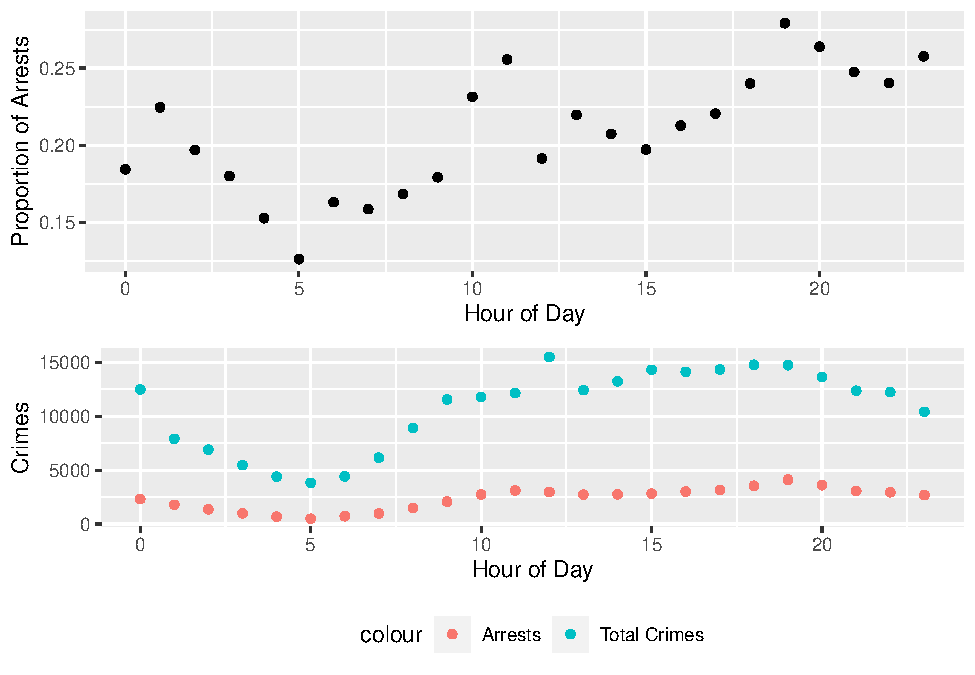
\includegraphics{rahil_notebook_files/figure-latex/unnamed-chunk-6-1.pdf}

\section{Binary Classification}

In this section we attempt to fit a binary classification model, to
predict given certain information whether the crime would lead to an
arrest or not. Choosing only to use 2019 data, due to scale of the data
set (leaving us with roughly 250,000 observations), as data recorded
after is affected strongly by COVID.

The features we choose to include in this model are:
\[\mathbf{x} = \texttt{(Domestic, Primary Type, Day, Time, Week Day, District})\]
We choose \texttt{Primary Type} over \texttt{FBI Code} to determine the
type of crime as during our EDA we found inconsistencies with the
classification of \texttt{FBI Code}. With \texttt{Primary Type}, we
merge uncommon levels of our factor variable into the level
\texttt{OTHER",\ in\ which\ we\ also\ include\ the\ pre-existing\ crime\ type}OTHER
OFFENSE''.

For temporal data we include \texttt{Week Day} as a factor variable,
encoding date using \texttt{Day} (1-365) and \texttt{Time} as a numeric
character between 0-1.

In order to include spatial information, we consider the
\texttt{District} variable. We observe that all districts experience
reasonable numbers of crimes to be incorporated into analysis, with the
exception of District 031.

While including more information might improve our models, during our
EDA we found the inclusion of highly correlated variables to improve the
model insignificantly while drastically increasing computational time.

\subsection{Logistic Regression}

\begin{Shaded}
\begin{Highlighting}[]
\FunctionTok{library}\NormalTok{(caret)}
\FunctionTok{library}\NormalTok{(doParallel)}
\end{Highlighting}
\end{Shaded}

\begin{verbatim}
## Loading required package: foreach
\end{verbatim}

\begin{verbatim}
## Loading required package: iterators
\end{verbatim}

\begin{verbatim}
## Loading required package: parallel
\end{verbatim}

\begin{Shaded}
\begin{Highlighting}[]
\FunctionTok{set.seed}\NormalTok{(}\DecValTok{30700}\NormalTok{) }\CommentTok{\# Setting seed for reproducibility}
\end{Highlighting}
\end{Shaded}

Using the package \texttt{doParallel} and \texttt{caret} we can easily
fit classification models. We define a control method which allows our
function to do 5-fold Cross Validation, using \texttt{doParallel} to do
the cross validation in parallel to decrease computational time. Setting
seeds for our cross-validation function to ensure reproducibility. The
function will return the model with the highest accuracy, however we can
see the accuracy for the other models in the cross validation process.

\begin{Shaded}
\begin{Highlighting}[]
\CommentTok{\#Create Seeds for the Cross Validation Function}
\NormalTok{seeds }\OtherTok{\textless{}{-}} \FunctionTok{vector}\NormalTok{(}\AttributeTok{mode =} \StringTok{"list"}\NormalTok{, }\AttributeTok{length =} \DecValTok{6}\NormalTok{)}
\ControlFlowTok{for}\NormalTok{(i }\ControlFlowTok{in} \DecValTok{1}\SpecialCharTok{:}\DecValTok{6}\NormalTok{) seeds[[i]] }\OtherTok{\textless{}{-}} \FunctionTok{sample.int}\NormalTok{(}\AttributeTok{n=}\DecValTok{1000}\NormalTok{, }\DecValTok{3}\NormalTok{)}

\CommentTok{\#Define Cross Validation Function}
\NormalTok{control }\OtherTok{\textless{}{-}} \FunctionTok{trainControl}\NormalTok{(}\AttributeTok{method =} \StringTok{\textquotesingle{}cv\textquotesingle{}}\NormalTok{, }\AttributeTok{number =} \DecValTok{5}\NormalTok{, }\AttributeTok{allowParallel =} \ConstantTok{TRUE}\NormalTok{, }\AttributeTok{seeds=}\NormalTok{seeds)}

\NormalTok{cl }\OtherTok{\textless{}{-}} \FunctionTok{makePSOCKcluster}\NormalTok{(}\FunctionTok{detectCores}\NormalTok{() }\SpecialCharTok{{-}} \DecValTok{1}\NormalTok{)}

\FunctionTok{registerDoParallel}\NormalTok{(cl)}

\CommentTok{\#Fitting Logistic Regression Classifier}
\NormalTok{log.model }\OtherTok{\textless{}{-}} \FunctionTok{train}\NormalTok{(Arrest }\SpecialCharTok{\textasciitilde{}}\NormalTok{ .,}
               \AttributeTok{data =}\NormalTok{ crimes,}
               \AttributeTok{trControl =}\NormalTok{ control,}
               \AttributeTok{method =} \StringTok{"glm"}\NormalTok{,}
               \AttributeTok{family=}\FunctionTok{binomial}\NormalTok{())}

\FunctionTok{stopCluster}\NormalTok{(cl)}
\end{Highlighting}
\end{Shaded}

\subsection{Support Vector Machines}

In this section we fit Support Vector Machines with the Radial Basis
Kernel (due to the unclear relationship between our predictors and
class).

As SVM models scale badly with data points we have to train our models
on samples of our data set (which has greater than \(250,000\) data
points). We will be fitting 3 SVM models, each using a different
sampling technique.

\begin{itemize}
    \item The first method is to take a proportional sample, which attempts to generate a sample where the proportion of each classes emulates the original data set.
    \item The next is known as 'Down Sampling' where we randomly sample the majority class till we have the same number of observations as the minority class.
    \item Similarly we will use the method known as 'Up Sampling', randomly samples (with replacement) the minority class until we have the same number of observations as the majority class.
\end{itemize}

It is clear than in our data there is a significant imbalance in the
class proportions.We see that only \(21.7%
\) of the data has \texttt{Arrest\ =\ TRUE}.

\begin{Shaded}
\begin{Highlighting}[]
\NormalTok{crimes }\SpecialCharTok{\%\textgreater{}\%}\NormalTok{ dplyr}\SpecialCharTok{::}\FunctionTok{count}\NormalTok{(Arrest)}
\end{Highlighting}
\end{Shaded}

\begin{verbatim}
## # A tibble: 2 x 2
##   Arrest      n
##   <fct>   <int>
## 1 FALSE  202086
## 2 TRUE    56068
\end{verbatim}

For our first SVM model, we will take a representative sample of roughly
13,000 data points. The \texttt{createDataPartition} function in
\texttt{caret} allows us to easily do this.

\begin{Shaded}
\begin{Highlighting}[]
\NormalTok{trainIndex }\OtherTok{\textless{}{-}} \FunctionTok{createDataPartition}\NormalTok{(crimes}\SpecialCharTok{$}\NormalTok{Arrest, }\AttributeTok{p =}\NormalTok{ .}\DecValTok{05}\NormalTok{, }
                                  \AttributeTok{list =} \ConstantTok{TRUE}\NormalTok{)}

\NormalTok{crimesTest }\OtherTok{\textless{}{-}}\NormalTok{ crimes[trainIndex}\SpecialCharTok{$}\NormalTok{Resample,]}

\NormalTok{crimesTest }\SpecialCharTok{\%\textgreater{}\%}\NormalTok{ dplyr}\SpecialCharTok{::}\FunctionTok{count}\NormalTok{(Arrest)}
\end{Highlighting}
\end{Shaded}

\begin{verbatim}
## # A tibble: 2 x 2
##   Arrest     n
##   <fct>  <int>
## 1 FALSE  10105
## 2 TRUE    2804
\end{verbatim}

Just like with the Logistic Regression Classifier we use the
\texttt{train} function from \texttt{caret} using our previously defined
train function - which has the exact same implementation for the SVMs we
fit. The \texttt{svmRadial} method uses \texttt{kernlab::sigest} to
determine a good predictor for \(\sigma\). It will then test multiple
values for Cost and will choose the one which maximizes accuracy. The
\texttt{train} function will work in this manner for the other 2 models
we train as well.

\begin{Shaded}
\begin{Highlighting}[]
\NormalTok{cl }\OtherTok{\textless{}{-}} \FunctionTok{makePSOCKcluster}\NormalTok{(}\FunctionTok{detectCores}\NormalTok{() }\SpecialCharTok{{-}} \DecValTok{1}\NormalTok{)}

\FunctionTok{registerDoParallel}\NormalTok{(cl)}

\CommentTok{\#Fitting SVM Model with a Proportional Sample}
\NormalTok{svm.model }\OtherTok{\textless{}{-}} \FunctionTok{train}\NormalTok{(Arrest }\SpecialCharTok{\textasciitilde{}}\NormalTok{ .,}
                   \AttributeTok{data =}\NormalTok{ crimesTest,}
                   \AttributeTok{trControl =}\NormalTok{ control,}
                   \AttributeTok{method =} \StringTok{\textquotesingle{}svmRadial\textquotesingle{}}\NormalTok{,}
                   \AttributeTok{family =} \FunctionTok{binomial}\NormalTok{(),}
                   \AttributeTok{allowParallel =} \ConstantTok{TRUE}\NormalTok{)}

\FunctionTok{stopCluster}\NormalTok{(cl)}
\end{Highlighting}
\end{Shaded}

As we will be taking a somewhat small sample of our whole data set to
train this model on, we will now try a method called down sampling, this
a method of sampling a data set in which we take all of the data points
from our lowest proportion class, and sample an equal amount of the
other proportions of the classes.

First we use the \texttt{downSample} function from \texttt{caret} this
takes a sample of our data set, giving us an equal sample of both
\texttt{Arrest\ =\ TRUE} and \texttt{Arrest\ =\ FALSE}.

\begin{Shaded}
\begin{Highlighting}[]
\NormalTok{down\_sample }\OtherTok{\textless{}{-}} \FunctionTok{downSample}\NormalTok{(}\AttributeTok{x =}\NormalTok{ crimes, }\AttributeTok{y =}\NormalTok{ crimes}\SpecialCharTok{$}\NormalTok{Arrest)}
\NormalTok{down\_sample }\SpecialCharTok{\%\textgreater{}\%} \FunctionTok{count}\NormalTok{(Arrest)}
\end{Highlighting}
\end{Shaded}

\begin{verbatim}
##   Arrest     n
## 1  FALSE 56068
## 2   TRUE 56068
\end{verbatim}

We see that the sample involves all the TRUE data points and gives a
random sample of our FALSE data points, we can now use the
\texttt{createDataPartition} function to take a representative sample of
\texttt{down\_sample} (of equal size to our other sample).

\begin{Shaded}
\begin{Highlighting}[]
\NormalTok{trainIndexD }\OtherTok{\textless{}{-}} \FunctionTok{createDataPartition}\NormalTok{(down\_sample}\SpecialCharTok{$}\NormalTok{Arrest, }\AttributeTok{p =} \FunctionTok{nrow}\NormalTok{(crimesTest)}\SpecialCharTok{/}\FunctionTok{nrow}\NormalTok{(down\_sample), }
                                 \AttributeTok{list =} \ConstantTok{TRUE}\NormalTok{)}

\NormalTok{crimesTestD }\OtherTok{\textless{}{-}}\NormalTok{ down\_sample[trainIndexD}\SpecialCharTok{$}\NormalTok{Resample,] }\SpecialCharTok{\%\textgreater{}\%} \FunctionTok{select}\NormalTok{(}\SpecialCharTok{{-}}\NormalTok{Class)}

\NormalTok{crimesTestD }\SpecialCharTok{\%\textgreater{}\%} \FunctionTok{count}\NormalTok{(Arrest)}
\end{Highlighting}
\end{Shaded}

\begin{verbatim}
##   Arrest    n
## 1  FALSE 6455
## 2   TRUE 6455
\end{verbatim}

\begin{Shaded}
\begin{Highlighting}[]
\NormalTok{cl }\OtherTok{\textless{}{-}} \FunctionTok{makePSOCKcluster}\NormalTok{(}\FunctionTok{detectCores}\NormalTok{() }\SpecialCharTok{{-}} \DecValTok{1}\NormalTok{)}

\FunctionTok{registerDoParallel}\NormalTok{(cl)}

\CommentTok{\#Training a SVM using down sampling}
\NormalTok{svm.modelD }\OtherTok{\textless{}{-}} \FunctionTok{train}\NormalTok{(Arrest }\SpecialCharTok{\textasciitilde{}}\NormalTok{ .,}
                   \AttributeTok{data =}\NormalTok{ crimesTestD,}
                   \AttributeTok{trControl =}\NormalTok{ control,}
                   \AttributeTok{method =} \StringTok{\textquotesingle{}svmRadial\textquotesingle{}}\NormalTok{,}
                   \AttributeTok{family =} \FunctionTok{binomial}\NormalTok{())}

\FunctionTok{stopCluster}\NormalTok{(cl)}
\end{Highlighting}
\end{Shaded}

There is another method of sampling in a similar vein to down sampling,
known as up sampling where we sample with replacement the non majority
classes until they are of the same length as the majority class in a
similar manner with down sampling we will train a model.

\begin{Shaded}
\begin{Highlighting}[]
\NormalTok{up\_sample }\OtherTok{\textless{}{-}} \FunctionTok{upSample}\NormalTok{(}\AttributeTok{x =}\NormalTok{ crimes, }\AttributeTok{y =}\NormalTok{ crimes}\SpecialCharTok{$}\NormalTok{Arrest)}
\NormalTok{up\_sample }\SpecialCharTok{\%\textgreater{}\%} \FunctionTok{count}\NormalTok{(Arrest)}
\end{Highlighting}
\end{Shaded}

\begin{verbatim}
##   Arrest      n
## 1  FALSE 202086
## 2   TRUE 202086
\end{verbatim}

\begin{Shaded}
\begin{Highlighting}[]
\FunctionTok{set.seed}\NormalTok{(}\DecValTok{1}\NormalTok{)}
\NormalTok{trainIndexU }\OtherTok{\textless{}{-}} \FunctionTok{createDataPartition}\NormalTok{(up\_sample}\SpecialCharTok{$}\NormalTok{Arrest, }\AttributeTok{p =} \FunctionTok{nrow}\NormalTok{(crimesTest)}\SpecialCharTok{/}\FunctionTok{nrow}\NormalTok{(up\_sample), }
                                 \AttributeTok{list =} \ConstantTok{TRUE}\NormalTok{)}

\NormalTok{crimesTestU }\OtherTok{\textless{}{-}}\NormalTok{ up\_sample[trainIndexU}\SpecialCharTok{$}\NormalTok{Resample,] }\SpecialCharTok{\%\textgreater{}\%} \FunctionTok{select}\NormalTok{(}\SpecialCharTok{{-}}\NormalTok{Class)}

\NormalTok{crimesTestU }\SpecialCharTok{\%\textgreater{}\%} \FunctionTok{count}\NormalTok{(Arrest)}
\end{Highlighting}
\end{Shaded}

\begin{verbatim}
##   Arrest    n
## 1  FALSE 6455
## 2   TRUE 6455
\end{verbatim}

\begin{Shaded}
\begin{Highlighting}[]
\NormalTok{cl }\OtherTok{\textless{}{-}} \FunctionTok{makePSOCKcluster}\NormalTok{(}\FunctionTok{detectCores}\NormalTok{() }\SpecialCharTok{{-}} \DecValTok{1}\NormalTok{)}

\FunctionTok{registerDoParallel}\NormalTok{(cl)}

\CommentTok{\#Training a SVM using up sampling}
\NormalTok{svm.modelU }\OtherTok{\textless{}{-}} \FunctionTok{train}\NormalTok{(Arrest }\SpecialCharTok{\textasciitilde{}}\NormalTok{ .,}
                   \AttributeTok{data =}\NormalTok{ crimesTestU,}
                   \AttributeTok{trControl =}\NormalTok{ control,}
                   \AttributeTok{method =} \StringTok{\textquotesingle{}svmRadial\textquotesingle{}}\NormalTok{,}
                   \AttributeTok{family =} \FunctionTok{binomial}\NormalTok{())}

\FunctionTok{stopCluster}\NormalTok{(cl)}
\NormalTok{svm.modelU}\SpecialCharTok{$}\NormalTok{results[}\FunctionTok{c}\NormalTok{(}\StringTok{\textquotesingle{}Accuracy\textquotesingle{}}\NormalTok{, }\StringTok{\textquotesingle{}Kappa\textquotesingle{}}\NormalTok{)]}
\end{Highlighting}
\end{Shaded}

\begin{verbatim}
##    Accuracy     Kappa
## 1 0.7316809 0.4633617
## 2 0.7316809 0.4633617
## 3 0.7302091 0.4604183
\end{verbatim}

\subsection{Model Performance}

To test the performance of our Models, we will simulate 10 proportional
(in respect to number of arrests), testing data sets. For each of these
testing sets we will some metrics. The metrics below will be ones
measured for each of models.

\[Accuracy = Pr(\hat{Y} = Y)\]
\[Sensitivity = Pr(\hat{Y} = 1 | Y = 1) = Pr(\text{True Positive})\]
\[Specificity = Pr(\hat{Y} = 0| Y = 0) = Pr(\text{True Negative})\]
\[\text{Balanced Accuracy} = \frac{Sensitivity + Specificity}{2}\]

An interesting benchmark for the usefulness of the model is the
No-Information Rate which is the accuracy if we just guess for each data
point is the largest proportion class. For the crimes data set that is
\(0.7828\), however this is not some foolproof benchmark, for example if
our goal is to predict to lowest proportion class consistently.

\begin{Shaded}
\begin{Highlighting}[]
\NormalTok{blank }\OtherTok{\textless{}{-}} \FunctionTok{data.frame}\NormalTok{(}\AttributeTok{Model =} \FunctionTok{as.character}\NormalTok{(), }\AttributeTok{ACC=}\FunctionTok{numeric}\NormalTok{(}\DecValTok{0}\NormalTok{),}\AttributeTok{SENS =} \FunctionTok{numeric}\NormalTok{(}\DecValTok{0}\NormalTok{), }\AttributeTok{SPEC =} \FunctionTok{numeric}\NormalTok{(}\DecValTok{0}\NormalTok{), }\AttributeTok{BALACC =} \FunctionTok{numeric}\NormalTok{(}\DecValTok{0}\NormalTok{)) }
\NormalTok{up }\OtherTok{\textless{}{-}}\NormalTok{ blank}
\NormalTok{down }\OtherTok{\textless{}{-}}\NormalTok{ blank}
\NormalTok{logistic }\OtherTok{\textless{}{-}}\NormalTok{ blank }
\NormalTok{repSVM }\OtherTok{\textless{}{-}}\NormalTok{ blank}

\CommentTok{\#Creating data frames of our metrics}
\ControlFlowTok{for}\NormalTok{ (testrow }\ControlFlowTok{in} \DecValTok{1}\SpecialCharTok{:}\DecValTok{10}\NormalTok{)\{}
\NormalTok{  sampIndex }\OtherTok{\textless{}{-}} \FunctionTok{createDataPartition}\NormalTok{(crimes}\SpecialCharTok{$}\NormalTok{Arrest, }\AttributeTok{p =}\NormalTok{ .}\DecValTok{025}\NormalTok{, }
                                  \AttributeTok{list =} \ConstantTok{TRUE}\NormalTok{)}
  
\NormalTok{  sampTest }\OtherTok{\textless{}{-}}\NormalTok{ crimes[sampIndex}\SpecialCharTok{$}\NormalTok{Resample,]}
  
\NormalTok{  u }\OtherTok{\textless{}{-}} \FunctionTok{confusionMatrix}\NormalTok{(}\AttributeTok{data =} \FunctionTok{predict}\NormalTok{(svm.modelU, }\AttributeTok{newdata =}\NormalTok{ sampTest),}
                       \AttributeTok{reference =}\NormalTok{ sampTest}\SpecialCharTok{$}\NormalTok{Arrest, }\AttributeTok{positive =} \StringTok{\textquotesingle{}TRUE\textquotesingle{}}\NormalTok{)}
\NormalTok{  d }\OtherTok{\textless{}{-}} \FunctionTok{confusionMatrix}\NormalTok{(}\AttributeTok{data =} \FunctionTok{predict}\NormalTok{(svm.modelD, }\AttributeTok{newdata =}\NormalTok{ sampTest),}
                       \AttributeTok{reference =}\NormalTok{ sampTest}\SpecialCharTok{$}\NormalTok{Arrest, }\AttributeTok{positive =} \StringTok{\textquotesingle{}TRUE\textquotesingle{}}\NormalTok{)}
\NormalTok{  l }\OtherTok{\textless{}{-}} \FunctionTok{confusionMatrix}\NormalTok{(}\AttributeTok{data =} \FunctionTok{predict}\NormalTok{(log.model, }\AttributeTok{newdata =}\NormalTok{ sampTest),}
                       \AttributeTok{reference =}\NormalTok{ sampTest}\SpecialCharTok{$}\NormalTok{Arrest, }\AttributeTok{positive =} \StringTok{\textquotesingle{}TRUE\textquotesingle{}}\NormalTok{)}
\NormalTok{  r }\OtherTok{\textless{}{-}} \FunctionTok{confusionMatrix}\NormalTok{(}\AttributeTok{data =} \FunctionTok{predict}\NormalTok{(svm.model, }\AttributeTok{newdata =}\NormalTok{ sampTest),}
                       \AttributeTok{reference =}\NormalTok{ sampTest}\SpecialCharTok{$}\NormalTok{Arrest, }\AttributeTok{positive =} \StringTok{\textquotesingle{}TRUE\textquotesingle{}}\NormalTok{)}
  
\NormalTok{  up[testrow, ] }\OtherTok{\textless{}{-}} \FunctionTok{c}\NormalTok{(}\StringTok{\textquotesingle{}UpSVM\textquotesingle{}}\NormalTok{,u[[}\StringTok{"overall"}\NormalTok{]][[}\StringTok{"Accuracy"}\NormalTok{]], u[[}\StringTok{"byClass"}\NormalTok{]][[}\StringTok{"Sensitivity"}\NormalTok{]],}
\NormalTok{               u[[}\StringTok{"byClass"}\NormalTok{]][[}\StringTok{"Specificity"}\NormalTok{]], u[[}\StringTok{"byClass"}\NormalTok{]][[}\StringTok{"Balanced Accuracy"}\NormalTok{]])}
  
\NormalTok{  down[testrow, ] }\OtherTok{\textless{}{-}} \FunctionTok{c}\NormalTok{(}\StringTok{\textquotesingle{}DownSVM\textquotesingle{}}\NormalTok{,d[[}\StringTok{"overall"}\NormalTok{]][[}\StringTok{"Accuracy"}\NormalTok{]], d[[}\StringTok{"byClass"}\NormalTok{]][[}\StringTok{"Sensitivity"}\NormalTok{]],}
\NormalTok{               d[[}\StringTok{"byClass"}\NormalTok{]][[}\StringTok{"Specificity"}\NormalTok{]], d[[}\StringTok{"byClass"}\NormalTok{]][[}\StringTok{"Balanced Accuracy"}\NormalTok{]])}
  
\NormalTok{  logistic[testrow, ] }\OtherTok{\textless{}{-}} \FunctionTok{c}\NormalTok{(}\StringTok{\textquotesingle{}LogReg\textquotesingle{}}\NormalTok{,l[[}\StringTok{"overall"}\NormalTok{]][[}\StringTok{"Accuracy"}\NormalTok{]], l[[}\StringTok{"byClass"}\NormalTok{]][[}\StringTok{"Sensitivity"}\NormalTok{]],}
\NormalTok{               l[[}\StringTok{"byClass"}\NormalTok{]][[}\StringTok{"Specificity"}\NormalTok{]], l[[}\StringTok{"byClass"}\NormalTok{]][[}\StringTok{"Balanced Accuracy"}\NormalTok{]])}
  
\NormalTok{  repSVM[testrow, ] }\OtherTok{\textless{}{-}} \FunctionTok{c}\NormalTok{(}\StringTok{\textquotesingle{}SVM\textquotesingle{}}\NormalTok{,r[[}\StringTok{"overall"}\NormalTok{]][[}\StringTok{"Accuracy"}\NormalTok{]], r[[}\StringTok{"byClass"}\NormalTok{]][[}\StringTok{"Sensitivity"}\NormalTok{]],}
\NormalTok{               r[[}\StringTok{"byClass"}\NormalTok{]][[}\StringTok{"Specificity"}\NormalTok{]], r[[}\StringTok{"byClass"}\NormalTok{]][[}\StringTok{"Balanced Accuracy"}\NormalTok{]])}
\NormalTok{\}}
\end{Highlighting}
\end{Shaded}

Below we have a table of the mean values of the metrics previously
defined for each model.

\begin{Shaded}
\begin{Highlighting}[]
\NormalTok{FullBinTest }\OtherTok{\textless{}{-}} \FunctionTok{rbind}\NormalTok{(up,down,logistic,repSVM) }\SpecialCharTok{\%\textgreater{}\%}  \FunctionTok{mutate}\NormalTok{(}\AttributeTok{Model =} \FunctionTok{as.factor}\NormalTok{(Model), }
                                                          \AttributeTok{ACC =} \FunctionTok{as.numeric}\NormalTok{(ACC), }
                                                          \AttributeTok{SENS =} \FunctionTok{as.numeric}\NormalTok{(SENS), }
                                                          \AttributeTok{SPEC =} \FunctionTok{as.numeric}\NormalTok{(SPEC), }
                                                          \AttributeTok{BALACC =} \FunctionTok{as.numeric}\NormalTok{(BALACC))}

\NormalTok{FullBinTest }\SpecialCharTok{\%\textgreater{}\%} \FunctionTok{group\_by}\NormalTok{(Model) }\SpecialCharTok{\%\textgreater{}\%} \FunctionTok{summarise}\NormalTok{(}\FunctionTok{across}\NormalTok{(}\FunctionTok{everything}\NormalTok{(), mean))}
\end{Highlighting}
\end{Shaded}

\begin{verbatim}
## # A tibble: 4 x 5
##   Model     ACC  SENS  SPEC BALACC
##   <fct>   <dbl> <dbl> <dbl>  <dbl>
## 1 DownSVM 0.767 0.662 0.796  0.729
## 2 LogReg  0.860 0.443 0.975  0.709
## 3 SVM     0.860 0.434 0.978  0.706
## 4 UpSVM   0.821 0.552 0.895  0.724
\end{verbatim}

\begin{Shaded}
\begin{Highlighting}[]
\NormalTok{ACCPlot }\OtherTok{\textless{}{-}} \FunctionTok{ggplot}\NormalTok{(FullBinTest, }\FunctionTok{aes}\NormalTok{(}\AttributeTok{x =}\NormalTok{ Model, }\AttributeTok{y =}\NormalTok{ ACC)) }\SpecialCharTok{+} \FunctionTok{geom\_boxplot}\NormalTok{() }\SpecialCharTok{+} 
  \FunctionTok{geom\_hline}\NormalTok{(}\AttributeTok{mapping =} \FunctionTok{aes}\NormalTok{(}\AttributeTok{yintercept =} \FloatTok{0.7828}\NormalTok{), }\AttributeTok{color =} \StringTok{\textquotesingle{}red\textquotesingle{}}\NormalTok{) }\SpecialCharTok{+} 
  \FunctionTok{labs}\NormalTok{(}\AttributeTok{title =} \StringTok{\textquotesingle{}Models and Accuracy\textquotesingle{}}\NormalTok{, }\AttributeTok{y =} \StringTok{\textquotesingle{}Accuracy\textquotesingle{}}\NormalTok{)}
\NormalTok{SENSPlot }\OtherTok{\textless{}{-}} \FunctionTok{ggplot}\NormalTok{(FullBinTest, }\FunctionTok{aes}\NormalTok{(}\AttributeTok{x =}\NormalTok{ Model, }\AttributeTok{y =}\NormalTok{ SENS)) }\SpecialCharTok{+} \FunctionTok{geom\_boxplot}\NormalTok{() }\SpecialCharTok{+}
  \FunctionTok{labs}\NormalTok{(}\AttributeTok{title =} \StringTok{\textquotesingle{}Models and Sensitivity\textquotesingle{}}\NormalTok{, }\AttributeTok{y =} \StringTok{\textquotesingle{}Sensitivity\textquotesingle{}}\NormalTok{)}
\NormalTok{SPECPlot }\OtherTok{\textless{}{-}} \FunctionTok{ggplot}\NormalTok{(FullBinTest, }\FunctionTok{aes}\NormalTok{(}\AttributeTok{x =}\NormalTok{ Model, }\AttributeTok{y =}\NormalTok{ SPEC)) }\SpecialCharTok{+} \FunctionTok{geom\_boxplot}\NormalTok{() }\SpecialCharTok{+}
  \FunctionTok{labs}\NormalTok{(}\AttributeTok{title =} \StringTok{\textquotesingle{}Models and Specificity\textquotesingle{}}\NormalTok{, }\AttributeTok{y =} \StringTok{\textquotesingle{}Specificity\textquotesingle{}}\NormalTok{)}
\NormalTok{BALACCPlot }\OtherTok{\textless{}{-}} \FunctionTok{ggplot}\NormalTok{(FullBinTest, }\FunctionTok{aes}\NormalTok{(}\AttributeTok{x =}\NormalTok{ Model, }\AttributeTok{y =}\NormalTok{ BALACC)) }\SpecialCharTok{+} \FunctionTok{geom\_boxplot}\NormalTok{() }\SpecialCharTok{+} 
  \FunctionTok{labs}\NormalTok{(}\AttributeTok{title =} \StringTok{\textquotesingle{}Models and Balanced Accuracy\textquotesingle{}}\NormalTok{, }\AttributeTok{y =} \StringTok{\textquotesingle{}Balanced Accuracy\textquotesingle{}}\NormalTok{)}

\FunctionTok{plot\_grid}\NormalTok{(ACCPlot,BALACCPlot , }\AttributeTok{nrow=}\DecValTok{1}\NormalTok{, }\AttributeTok{greedy =} \ConstantTok{TRUE}\NormalTok{)}
\end{Highlighting}
\end{Shaded}

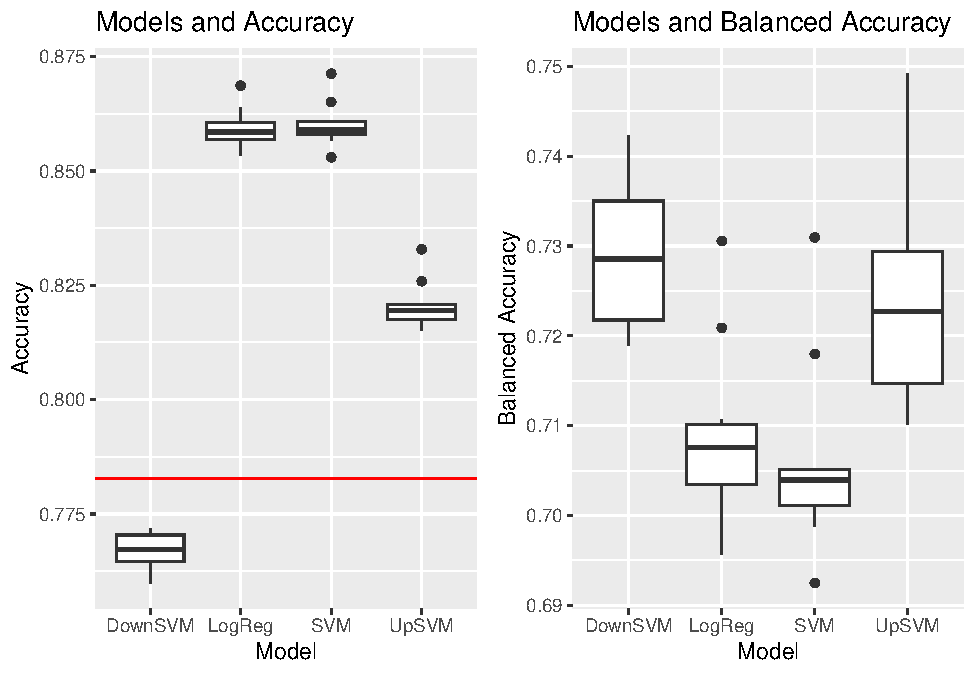
\includegraphics{rahil_notebook_files/figure-latex/unnamed-chunk-20-1.pdf}

\begin{Shaded}
\begin{Highlighting}[]
\FunctionTok{plot\_grid}\NormalTok{(SPECPlot, SENSPlot, }\AttributeTok{nrow=}\DecValTok{1}\NormalTok{, }\AttributeTok{greedy =} \ConstantTok{TRUE}\NormalTok{)}
\end{Highlighting}
\end{Shaded}

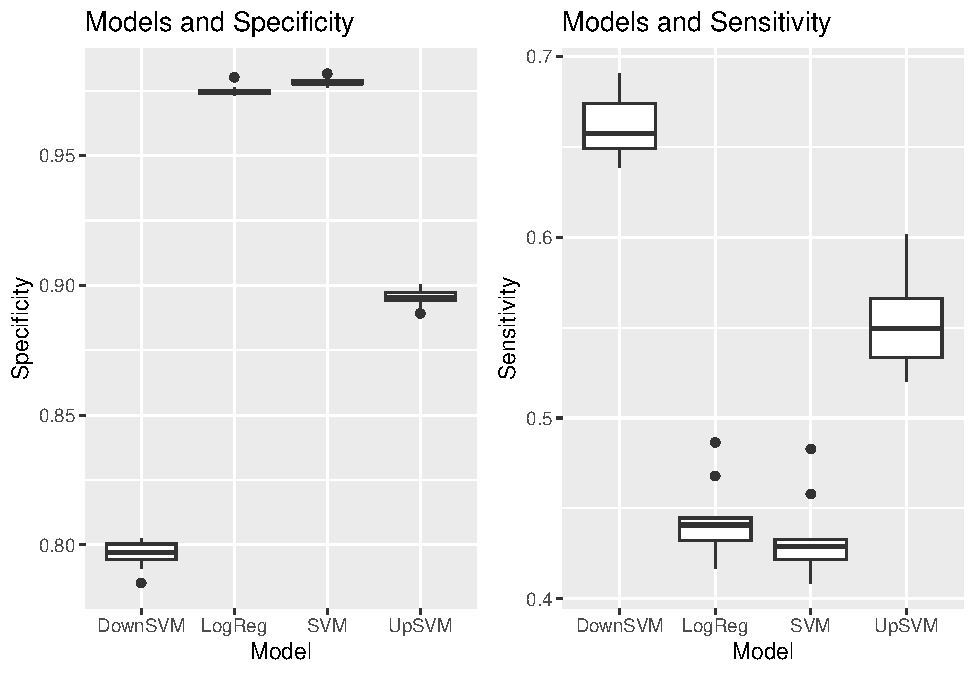
\includegraphics{rahil_notebook_files/figure-latex/unnamed-chunk-20-2.pdf}

We can see that both the proportional SVM Model and Logistic Model
performed very similarly, both with high accuracy and specificity, this
is to be expected, as both models were trained and tested with far more
\texttt{FALSE} data points. We can see that with the trade-off being in
sensitivity, both performing poorly at distinguishing positive data
points.

Another important point, is that we might have expected the SVM model to
perform better than the Logistic Regression Model, due to it's abilities
to take into account non-linear relationships; however, we can see they
performed very similarly in nearly all aspects, this is probably due to
SVM being trained on only \(5\%\) of the 2019 data set while our
Logistic Model was trained on the full 2019 data set.

As expected up and down sampling had a positive affect on the
sensitivity of the model due to the training data involving a larger
proportion of \texttt{TRUE} values. If we look at the down sampled
model, we see that the high sensitivity gives a large trade off with
specificity and accuracy (pushing it below the no information rate),
this model is far more likely than the other models to give a false
positive. This could be due to the down sample involving sampling the
\texttt{FALSE} data points possibly giving a less informative sample.

Compared to down sampling, up sampling did not increase the sensitivity
as much, but instead found a more balanced trade off with specificity
and accuracy - this is interesting given that both models were trained
on the same amount of \texttt{TRUE} and \texttt{FALSE} data points,
further analysis would be needed to determine whether this was due to an
intrinsic property of the sampling technique or just due to randomness.

The better balanced accuracy of the up and down sampled models, shows
that accuracy of the Logistic and proportional models comes heavily from
it's lack of sensitivity combined with the imbalanced class proportions,
and that depending on what the goal of our models it might be preferable
to pick a less overall accurate model.

\end{document}
